\section{Prioritizing What to Work On}

\subsection{System Design Example}

Given a data set of emails, we could construct a vector for each email. Each entry in this vector represents a word. The vector normally contains 10,000 to 50,000 entries gathered by finding the most frequently used words in our data set. If a word is to be found in the email, we would assign its respective entry a 1, else if it is not found, that entry would be a 0. Once we have all our x vectors ready, we train our algorithm and finally, we could use it to classify if an email is a spam or not.

\begin{figure}[h!]
	\centering
	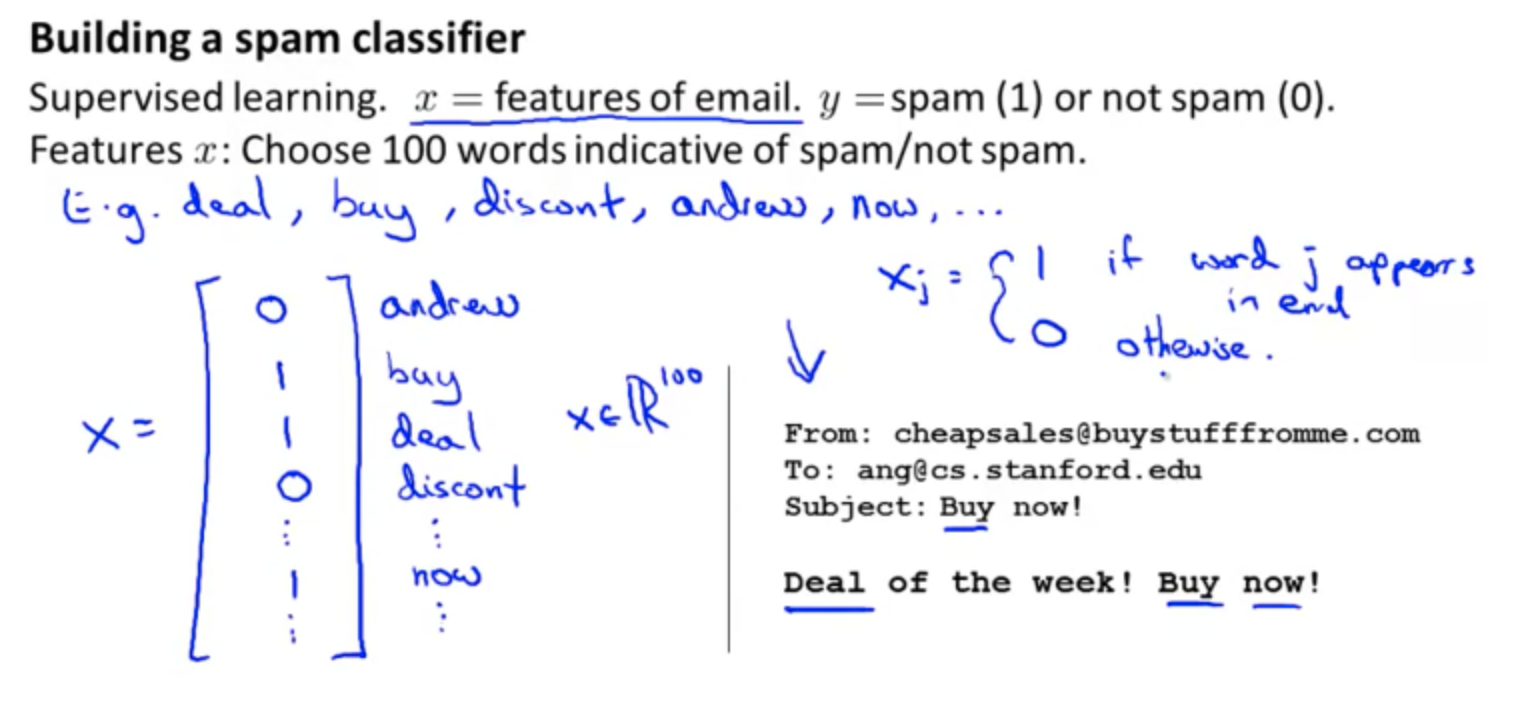
\includegraphics[width=1\textwidth]{fig/spam}
	\caption{Spam vector explanation}
\end{figure}

So how could you spend your time to improve the accuracy of this classifier?\\

\begin{itemize}
\item Collect lots of data (for example "honeypot" project but doesn't always work)
\item Develop sophisticated features (for example: using email header data in spam emails)
\item Develop algorithms to process your input in different ways (recognizing misspellings in spam).
\end{itemize}

It is difficult to tell which of the options will be most helpful.

\section{Error Analysis}

The recommended approach to solving machine learning problems is to:

\begin{enumerate}
\item Start with a simple algorithm, implement it quickly, and test it early on your cross validation data.
\item Plot learning curves to decide if more data, more features, etc. are likely to help.
\item Manually examine the errors on examples in the cross validation set and try to spot a trend where most of the errors were made.
\end{enumerate}

%For example, assume that we have 500 emails and our algorithm misclassifies a 100 of them. We could manually analyze the 100 emails and categorize them based on what type of emails they are. We could then try to come up with new cues and features that would help us classify these 100 emails correctly. Hence, if most of our misclassified emails are those which try to steal passwords, then we could find some features that are particular to those emails and add them to our model. We could also see how classifying each word according to its root changes our error rate.\\
%
%It is very important to get error results as a single, numerical value. Otherwise it is difficult to assess your algorithm's performance. For example if we use stemming, which is the process of treating the same word with different forms (fail/failing/failed) as one word (fail), and get a 3\% error rate instead of 5\%, then we should definitely add it to our model. However, if we try to distinguish between upper case and lower case letters and end up getting a 3.2\% error rate instead of 3\%, then we should avoid using this new feature. Hence, we should try new things, get a numerical value for our error rate, and based on our result decide whether we want to keep the new feature or not.
%
%\section{Skewed data}
%
%A data is called as skewed when curve appears distorted or skewed either to the left or to the right, in a statistical distribution. In a normal distribution, the graph appears symmetry meaning that there are about as many data values on the left side of the median as on the right side.\\
%
%In case of normal distribution, the mean, median and model are approximately closer. These three are all measures of the center of a data. The skewness of the data can be determined by how these quantities are related to one another.\\
%
%\subsection{Error metrics for skewed classes}
%
%Consider the problem of cancer classification, where we have features of medical patients and we want to decide whether or not they have cancer. So this is like the malignant versus benign tumor classification.\\
%
%Let's say \textbf{y equals 1} if the patient has cancer and \textbf{y equals 0} if they do not. We have trained the progression classifier and let's say we test our classifier on a test set and find that we get 1 percent error. So, we're making 99\% correct diagnosis. Seems like a really impressive result. We're correct 99\% percent of the time.\\
%
%But now, let's say we find out that only 0.5 percent of patients in our training test sets actually have cancer. So only half a percent of the patients that come through our screening process have cancer. In this case, the 1\% error no longer looks so impressive.\\
%
%So this setting of when the ratio of positive to negative examples is very close to one of two extremes, where, in this case, the number of positive examples is much, much smaller than the number of negative examples because y equals one so rarely, this is what we call the case of skewed classes.\\
%
%We just have a lot more of examples from one class than from the other class. And by just predicting y equals 0 all the time, or maybe our predicting y equals 1 all the time, an algorithm can do pretty well. So the problem with using classification error or classification accuracy as our evaluation metric is the following.\\
%
%Let's say you have one joining algorithm that's getting 99.2\% accuracy. So, that's a 0.8\% error. Let's say you make a change to your algorithm and you now are getting 99.5\% accuracy. That is 0.5\% error.\\
%
%If you have very skewed classes it becomes much harder to use just classification accuracy, because you can get very high classification accuracies or very low errors, and it's not always clear if doing so is really improving the quality of your classifier because predicting y equals 0 all the time doesn't seem like a particularly good classifier.\\
%Start transcript at 3 minutes 53 seconds3:53
%But just predicting y equals 0 more often can bring your error down to, you know, maybe as low as 0.5%. When we're faced with such a skewed classes therefore we would want to come up with a different error metric or a different evaluation metric. One such evaluation metric are what's called precision recall.
%Start transcript at 4 minutes 15 seconds4:15
%Let me explain what that is.
%Start transcript at 4 minutes 17 seconds4:17
%Let's say we are evaluating a classifier on the test set. For the examples in the test set the actual
%Start transcript at 4 minutes 25 seconds4:25
%class of that example in the test set is going to be either one or zero, right, if there is a binary classification problem.
%Start transcript at 4 minutes 33 seconds4:33
%And what our learning algorithm will do is it will, you know, predict some value for the class and our learning algorithm will predict the value for each example in my test set and the predicted value will also be either one or zero.
%Start transcript at 4 minutes 50 seconds4:50
%So let me draw a two by two table as follows, depending on a full of these entries depending on what was the actual class and what was the predicted class. If we have an example where the actual class is one and the predicted class is one then that's called
%Start transcript at 5 minutes 7 seconds5:07
%an example that's a true positive, meaning our algorithm predicted that it's positive and in reality the example is positive. If our learning algorithm predicted that something is negative, class zero, and the actual class is also class zero then that's what's called a true negative. We predicted zero and it actually is zero.
%Start transcript at 5 minutes 27 seconds5:27
%To find the other two boxes, if our learning algorithm predicts that the class is one but the
%Start transcript at 5 minutes 34 seconds5:34
%actual class is zero, then that's called a false positive.
%Start transcript at 5 minutes 39 seconds5:39
%So that means our algorithm for the patient is cancelled out in reality if the patient does not.
%Start transcript at 5 minutes 44 seconds5:44
%And finally, the last box is a zero, one. That's called a false negative because our algorithm predicted zero, but the actual class was one.
%Start transcript at 5 minutes 57 seconds5:57
%And so, we have this little sort of two by two table based on what was the actual class and what was the predicted class.
%Start transcript at 6 minutes 7 seconds6:07
%So here's a different way of evaluating the performance of our algorithm. We're going to compute two numbers. The first is called precision - and what that says is,
%Start transcript at 6 minutes 17 seconds6:17
%of all the patients where we've predicted that they have cancer,
%Start transcript at 6 minutes 20 seconds6:20
%what fraction of them actually have cancer?
%Start transcript at 6 minutes 24 seconds6:24
%So let me write this down, the precision of a classifier is the number of true positives divided by
%Start transcript at 6 minutes 32 seconds6:32
%the number that we predicted
%Start transcript at 6 minutes 37 seconds6:37
%as positive, right?
%Start transcript at 6 minutes 39 seconds6:39
%So of all the patients that we went to those patients and we told them, "We think you have cancer." Of all those patients, what fraction of them actually have cancer? So that's called precision. And another way to write this would be true positives and then in the denominator is the number of predicted positives, and so that would be the sum of the, you know, entries in this first row of the table. So it would be true positives divided by true positives. I'm going to abbreviate positive as POS and then plus false positives, again abbreviating positive using POS.
%Start transcript at 7 minutes 20 seconds7:20
%So that's called precision, and as you can tell high precision would be good. That means that all the patients that we went to and we said, "You know, we're very sorry. We think you have cancer," high precision means that of that group of patients most of them we had actually made accurate predictions on them and they do have cancer.
%Start transcript at 7 minutes 38 seconds7:38
%The second number we're going to compute is called recall, and what recall say is, if all the patients in, let's say, in the test set or the cross-validation set, but if all the patients in the data set that actually have cancer,
%Start transcript at 7 minutes 52 seconds7:52
%what fraction of them that we correctly detect as having cancer. So if all the patients have cancer, how many of them did we actually go to them and you know, correctly told them that we think they need treatment.
%Start transcript at 8 minutes 5 seconds8:05
%So, writing this down, recall is defined as the number of positives, the number of true positives, meaning the number of people that have cancer and that we correctly predicted have cancer
%Start transcript at 8 minutes 20 seconds8:20
%and we take that and divide that by, divide that by the number of actual positives,
%Start transcript at 8 minutes 31 seconds8:31
%so this is the right number of actual positives of all the people that do have cancer. What fraction do we directly flag and you know, send the treatment.
%Start transcript at 8 minutes 40 seconds8:40
%So, to rewrite this in a different form, the denominator would be the number of actual positives as you know, is the sum of the entries in this first column over here.
%Start transcript at 8 minutes 50 seconds8:50
%And so writing things out differently, this is therefore, the number of true positives, divided by
%Start transcript at 8 minutes 59 seconds8:59
%the number of true positives
%Start transcript at 9 minutes 2 seconds9:02
%plus the number of
%Start transcript at 9 minutes 6 seconds9:06
%false negatives.
%Start transcript at 9 minutes 9 seconds9:09
%And so once again, having a high recall would be a good thing.
%Start transcript at 9 minutes 14 seconds9:14
%So by computing precision and recall this will usually give us a better sense of how well our classifier is doing.
%Start transcript at 9 minutes 21 seconds9:21
%And in particular if we have a learning algorithm that predicts y equals zero all the time, if it predicts no one has cancer, then this classifier will have a recall equal to zero, because there won't be any true positives and so that's a quick way for us to recognize that, you know, a classifier that predicts y equals 0 all the time, just isn't a very good classifier. And more generally, even for settings where we have very skewed classes, it's not possible for an algorithm to sort of "cheat" and somehow get a very high precision and a very high recall by doing some simple thing like predicting y equals 0 all the time or predicting y equals 1 all the time. And so we're much more sure that a classifier of a high precision or high recall actually is a good classifier, and this gives us a more useful evaluation metric that is a more direct way to actually understand whether, you know, our algorithm may be doing well.
%Start transcript at 10 minutes 21 seconds10:21
%So one final note in the definition of precision and recall, that we would define precision and recall, usually we use the convention that y is equal to 1, in the presence of the more rare class. So if we are trying to detect. rare conditions such as cancer, hopefully that's a rare condition, precision and recall are defined setting y equals 1, rather than y equals 0, to be sort of that the presence of that rare class that we're trying to detect. And by using precision and recall, we find, what happens is that even if we have very skewed classes, it's not possible for an algorithm to you know, "cheat" and predict y equals 1 all the time, or predict y equals 0 all the time, and get high precision and recall. And in particular, if a classifier is getting high precision and high recall, then we are actually confident that the algorithm has to be doing well, even if we have very skewed classes.
%Start transcript at 11 minutes 18 seconds11:18
%So for the problem of skewed classes precision recall gives us more direct insight into how the learning algorithm is doing and this is often a much better way to evaluate our learning algorithms, than looking at classification error or classification accuracy, when the classes are very skewed.